\documentclass[sigplan,10pt]{acmart}
\pagestyle{plain}

\title{400 GB/E}
\author{Markuze Alex}
\date{September 2018}

\newcommand{\oursys}{netalloc }

\begin{document}

\maketitle
\section{Introduction}
We evaluate , the effects of a dedicated memory allocator on the Linux network stack at 100Gb/s and beyond.
We propose several optimizations which we evaluate rigorously in the next sections. We add a sclable cache for 64KB chunks of memory. The goal of this cache is to shortcut the cumbersome buddy allocator, gaining faster allocation on a single core and minimize contention on multicore. The cache is a generic magazine allocator.
The second optimization we use is adding a page\_frag based, byte grained memory allocator. The page\_frag allocator optimizes cache access patterns.
We also theorize that by using huge pages we can optimize the use of TLB and thus farther optimize the cycles/byte value.
Throughout this work, we refer to the modified kernel with the set of optimizations as \oursys.

Possible contributions listed in table \ref{tab:contributions}.
Additional open issues with small impacts listed in table \ref{tab:open_issues}.
\begin{table}[b]
\centering
\begin{tabular}{l|l}
contribution & impact \\\hline
1. locking issues in UDP TX & trivial\\
2. dedicated allocator & carefull wording needed\\
3. memory wall @400Gb/s & some solution needed\\
4. magical cache & no such thing...\\
5. UDP drops & not clear what that is.\\
\hline
\end{tabular}
\caption{\label{tab:contributions}Contribution}
\end{table}

\newpage

\section{Evaluation}
This section describes the in-depth analysis of 16 micro-benchmark experiments.
The experiments are partitioned into for sections; single core/multi-core and TCP/UDP.
On single core we evaluate TX/RX and RR on multi-core we evaluate TX/RX and Bi-Directional traffic.

\subsection{Summery of Results}
Tables ~\ref{tab:exec-single} and summersize the micro-benchmark results and analysis.
\begin{table*}
\centering
\begin{tabular}{l|c|c|c}
Experiment & vanilla & \oursys & reason\\\hline
Single UDP TX (Gb/s)& 44 & 52 (+18\%) &  instructions per packet\\
Single UDP RX & 90 & 52 & Faulty experiment\\
Single UDP RR (60B pps)& 186k & 195k(+4.8\%) & see discussion\\\hline
Single TCP TX (Gb/s)& 60.33 & 62.45 (+3.5\%) & Need manual inspection\\
Single TCP RX (Gb/s)& 55.3 & 56.48 (+2.7\%)& slightly better IPC\\
Single TCP RR (pps)& 176.6 & 185.2 (+5.1\%)& instructions per packet\\\hline
\end{tabular}
\caption{\label{tab:exec-single}Single core results breakdown.}
\end{table*}
\begin{table*}
\centering
\begin{tabular}{l|c|c|c}
Experiment & vanilla & \oursys & reason\\\hline
Multi UDP TX (Gb/s|CPU)& 147 | 100\% & 200 | 50\% &  Locking issues in vanilla\\
Multi UDP RX (Gb/s|CPU)& 200 | 40\%  & 200 | 40\% & Equal results\\
Multi UDP BI (Gb/s|CPU)& 240 | 100\% & 360 | 88\% &Locking in vanilla, \oursys limited by mem BW\\\hline
Multi TCP TX (Gb/s)& 187.41|39.7\% & 187.7|37.37\% & (+6.4\%)better instructions per packet - (alloc\_skb)\\
Multi TCP RX (Gb/s)& 200|46\% & 200|46\%& Equal results\\
Multi TCP BI (pps)& 350|64.13\% & 350|61.29\%& Not clear why 400Gb/s not reached\\\hline
\end{tabular}
\caption{\label{tab:exec-multi}Multi-core results breakdown.}
\end{table*}

\subsection{Single-core UDP}
All single core tests are aimed to utilize 100\% of the CPU. In UDP-TX we have a single netperf flow sending 63KB datagrams. Using a dedicated memory allocator, boosts performance by 17.4\% in single core UDP TX experiment.

\begin{figure}
\centering
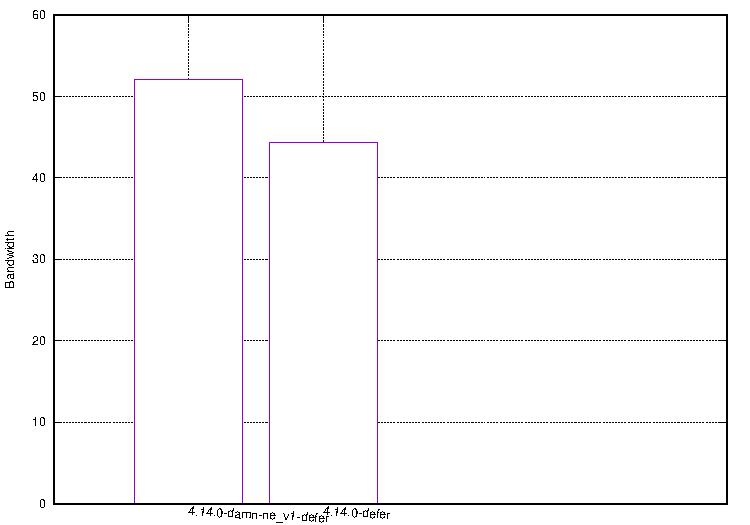
\includegraphics[width=0.5\textwidth]{figures/single_udp_tx_Bandwidth.pdf}
\caption{\label{fig:s-u-tx} Dan, I know that the text on the graph is too small. Single-core UDP TX.}
\end{figure}

\begin{figure}
\centering
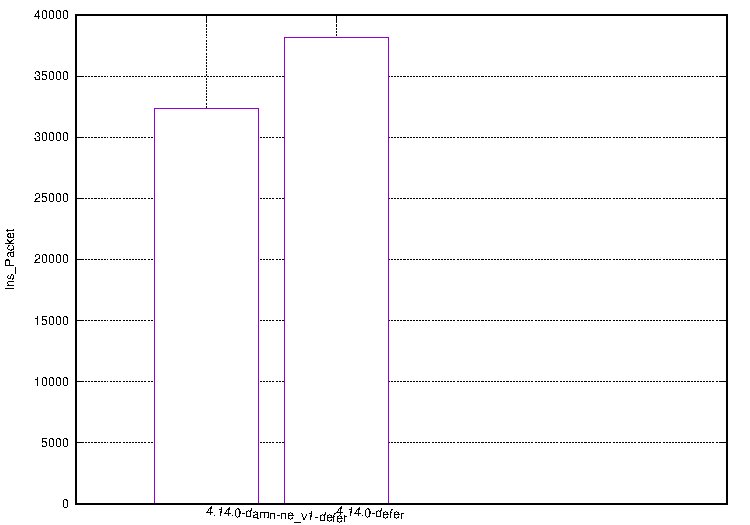
\includegraphics[width=0.5\textwidth]{figures/single_udp_tx_Ins_Packet.pdf}
\caption{\label{fig:s-u-tx-ipp} Single-core UDP TX, Instructions per packet.}
\end{figure}

In the case of single UDP TX, the main benefit is from faster allocation API. In figure \ref{fig:s-u-tx-ipp} we see the number of instructions per packet. The instructions per packet has the inverse ratio to the B/W, with 3798 vs 3235 cycles to vanilla and \oursys respectively. Curiously, both kernel versions had an almost identical number of cycles per second at 2.6e+9. In table \ref{tab:s-u-tx-funcs} we see the break down of cycles per packet. It seems that the major bulk of the 563 cycles that are saved by \oursys per packet come from the myriad of small functions removed from the allocation path. The path a pakcet takes in the vanilla kernel has 224 functions than in \oursys. 
\newline
Conclusion, although the system with \oursys seems to show better l2 and llc utilization(not seen in the above discussion).
The instructions per packet seem to provide the correct answer.

\begin{table}
\centering
\begin{tabular}{l|r|r}
Function & \oursys (3235)& vanilla (3798)\\\hline
csum\_partial\_copy\_generic & 43.85\% (1419) & 35.2\% (1337)\\
\_raw\_spinlock (\_\_dev\_queue\_xmit) & 4.75\% (153) & 4.45\% (169)\\
mlx5\_xmit & 3.43\% (111) & 2.52\% (96)\\
get\_page\_from\_free\_list & - & 2.43\% (92)\\
ip\_append\_data & 1.95\% (63) & 1.66\% (63)\\
alloc\_skb & 1.92\% (62) & 1.28\% (49)\\
ip\_finish\_output2 & 1.77\% (57) & 1.60\% (61)\\
mlx5\_poll\_tx\_cq & 1.64\% (53) & 1.40\% (53)\\
\_\_free\_pages\_ok & - & 1.37\% (52)\\
other & 59.31\% (1316) & 51.91\% (1826)
\end{tabular}
\caption{\label{tab:s-u-tx-funcs}Function breakdown.}
\end{table}

\subsection{Single UDP RR}
The answer is a balance between better IPC and higher(!) instructions per packet. The higher instructions per packet is due do higher interrupt count. Faster processing leads to NAPI failing to keep up (need coraboration, with irq count and packet/irq).  
\subsection{UDP Losses}
Previously, we have seen that while, the udp sender is sending 100Gb/s of BW the receiver is seeing effectively 0 bytes in userspace. This phenomena was always observed, regardless of whether the netserver cpu was shared with the NAPI/irq cpu or not.

State I:  vanila 4.17: 
device driver reports 98Gb/s packets sent.
/proc/net/dev* reports high numbers of rx-drop packets.
netserver reports tens of Mb/s received. 

state I fix: Apparently  there is  a NET\_FLOW\_LIMIT**, which was dropping our packets.
There is a bit mask that controls whether the flow limit is active or not, but the only thing that helped was compiling the kernel w/o this option.

Result: The counter for rx-dropp was no longer rising. 

State II: vanila 4.17 w/o net\_flow\_limit.
device driver reports 98Gb/s packets sent.
netserver reports tens of Mb/s received.
dropwatch*** reports ip\_defrag as the main "hub" for dropped packets.

state II fix: There were several changes introduced between 4.16 and 4.17. Eric Dumazet, from Google was working DDOS prevention, where ip\_defrag was the target.
The fix was; increasing the number of buckets:
sudo sh -c "echo 16000000000 >/proc/sys/net/ipv4/ipfrag\_high\_thresh"
Result: 
Driver started reporting on ~50Gb/s received packets while netserver was seeing about 25Gb/s. Due to packets lost in transit, ip\_defrag was now dropping packets that couldn't be reassembled. And yes, pause parameters are configured both on the sender and the receiver. The driver was now slower than the network and packets would get lost. 

fix II: I've modified the test to send 8KB udp packets, more system calls but no need to defrag the packets.

Result: Driver started reporting 42Gb/s received, with netserver reporting 38Gb/s.
dropwatch was now pointing to udp\_enqueue. Increasing the receive socket size
brought the netserver report up to 42Gb/s.
The short version of the above is that three things needed to maintain sane UDP RX results. The first thing that must be fixed is the NET\_FLOW\_LIMIT issue, the second thing is the size of received packets and the third is the size of the UDP socket.
The open question is; weather, its possible in software to decrease the number of lost fragments in flight. With PFC on this shouldn't have been an issue.

With DAMN, nothing seems to help. The RX counetrs show 95Gb/s, but about 90\% of those are dropped at \newline udp\_queue\_rcv\_skb. /proc/net/snmp is showing InErrors on RevbufErrors, this is inherent to ENOMEM error in \newline \_\_udp\_queue\_rcv\_skb. The difference stems from the speed of freed/recycled memory. The difference is seen in the delta between rx\_packets and rx\_packets\_phy, in our experiments the discrepancy is found in rx\_out\_of\_buffer ethtool counter, namely those packets that were dropped by the driver due to a lack of memory.  
\subsection{UDP}
\begin{itemize}
    \item Performance degradation at 4.18
    \begin{itemize}
        \item UDP RX effective RX is 50Mb/s
        \item UDP TX is 30GB/s vs 45Gb/s in 4.14
    \end{itemize}
    \item Damn with fragments - decreasing the sock size increases performance
    
\end{itemize}
Next Questions:
\begin{itemize}
    \item 64KB RX on Damn, where are the packets lost?
    \item budget limiting.
    \item schedule napi on TX, no IRQ.
\end{itemize}
\subsection{proc utilities}
https://www.kernel.org/doc/Documentation/sysctl/net.txt.
Q: Would, experiments with netdev\_budget\_usecs balance userspace/napi better.
Lowering usec to 50 usec and budget to 4, has no effect.
\subsection{IRQ observations}
TX traffic, TCP and UDP, generates around 50K irqs per sec. This is due to the fact that only RX packets are counted for napi budget. TCP RX generates around 25K irqs per second, with 30 packets handled on average.  
\subsection{More Questions}
Possible things that maybe beneficial to look at, table \ref{tab:open_issues}.
\begin{table*}
\centering
\begin{tabular}{l|l}
Issue & difficulty/impact \\\hline
Huge pages in \oursys & Few days of work expected <+5\% improved performance \\
New Theory: Add triger to NAPI call with TX Ring watermarks? & Awsome for TX and should also work for TCP\\
ad hoc NAPI budget & minor but could be interesting\\
TCP flows & why more than one flow needed to saturate single core?\\
Is prefetch usefull&\\
Inline functions & a known issue in the Linux community\\
UDP fragment losses & Not sure there is a resolution in SW\\
lock in TX queue & if were dealing with locks already...\\
coalescing & with higher rates may be its time to revisit?\\
Is xmit more used? & batching in send, could show up to +5\%\\
ad hoc driver memory reuse & motivation?\\
PFC & PFC has an impact on TCP performance, never looked at why\\
\hline
\end{tabular}


\caption{\label{tab:open_issues}Open issues}
\end{table*}

\begin{figure*}
    \centering
    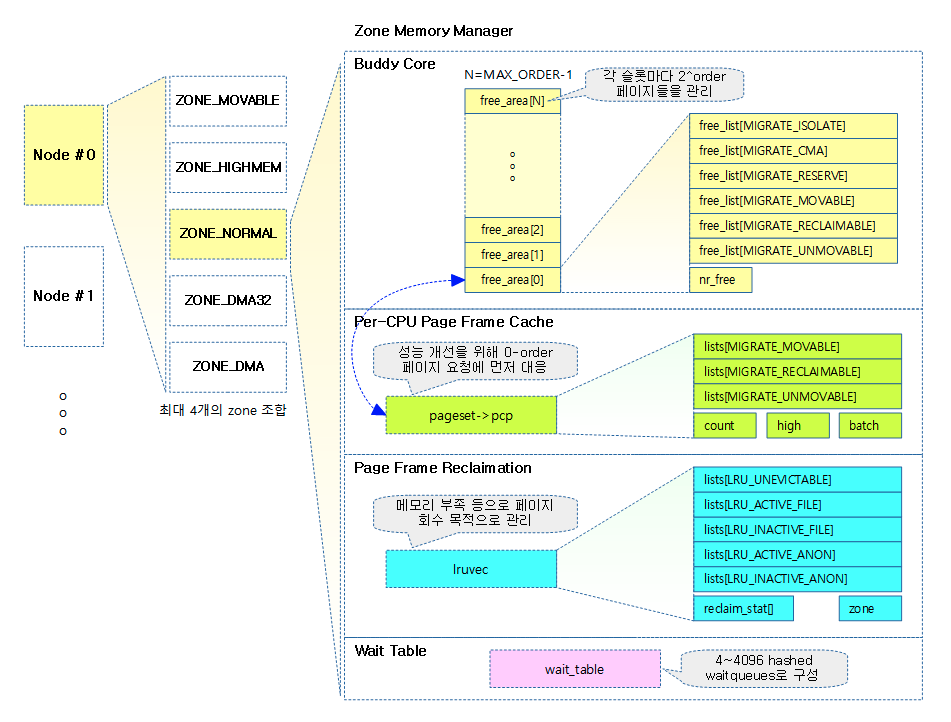
\includegraphics[width=1\textwidth]{figures/zoned_memory.png}
    \caption{Zoned memory allocator}
    \label{fig:zoned_memory_alloc}
\end{figure*}
\settopmatter{printfolios=true}
\renewcommand\footnotetextcopyrightpermission[1]{}
\end{document}
